\section{Exercise 2: An application of MCFP: rectilinear planar embedding}

\begin{figure*}
  \label{fig:rect-emb}

  \begin{center}
  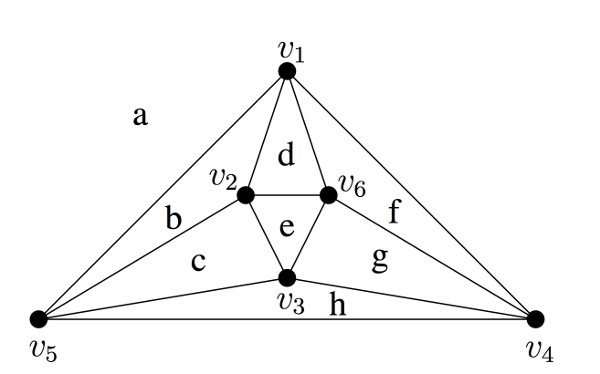
\includegraphics[scale=0.3]{img/fig2b.png}
  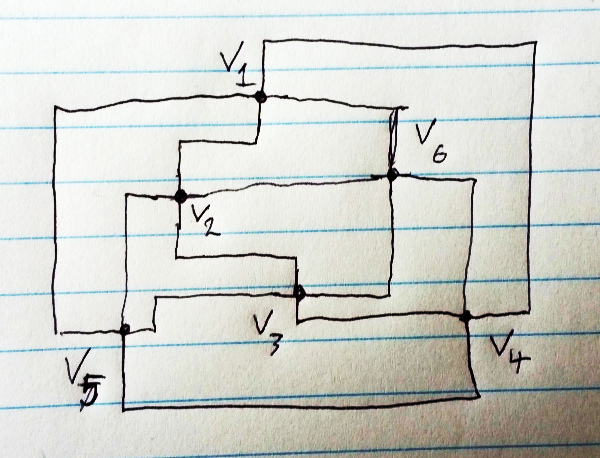
\includegraphics[scale=0.3]{img/ex21.png}
  \end{center}
  
  \caption{Figure 2 (b) from the practice set (left) and a sketch of its rectilinear embedding (right).}
\end{figure*}

\subsection{Exercise 2.1}

Listing only the values of $z_{fg}$ where $f$ and $g$ share an edge,
and on the values of $x_{vf}$ where $v$ is a corner edge of $f$.

\begingroup
\newcommand\zfg[3]{z_{ #1 #2} &= #3}
\newcommand\xvf[3]{x_{ #1 #2} &= #3}
\begin{minipage}{0.45\columnwidth}
\begin{align*}
  \zfg a b 0 \\
  \zfg a c 0 \\
  \zfg a e 0 \\
  \zfg b a 2 \\
  \zfg b c 1 \\
  \zfg b d 1 \\
  \zfg c a 1 \\
  \zfg c b 1 \\
  \zfg c d 0 \\
  \zfg d b 1 \\
  \zfg d c 0 \\
  \zfg d e 2 \\
  \zfg e a 4 \\
  \zfg e d 0
\end{align*}
\end{minipage}
\begin{minipage}{0.45\columnwidth}
\begin{align*}
  \xvf a 1 0 \\
  \xvf a 3 1 \\
  \xvf a 5 1 \\
  \xvf a 6 1 \\
  \xvf a 7 0 \\
  \xvf b 1 1 \\
  \xvf b 2 0 \\
  \xvf b 6 1 \\
  \xvf c 1 1 \\
  \xvf c 2 1 \\
  \xvf c 3 1 \\
  \xvf d 2 1 \\
  \xvf d 3 1 \\
  \xvf d 4 {-1} \\
  \xvf d 6 1 \\
  \xvf e 3 1 \\
  \xvf e 4 1 \\
  \xvf e 5 {-1} \\
  \xvf e 6 1 \\
  \xvf e 7 0
\end{align*}
\end{minipage}
\endgroup

(A/N: This should \emph{probably} have been a table. Sorry.)

See Figure~\ref{fig:rect-emb} for the rectilinear embedding.

\subsection{Exercise 2.2}

The outer boundary cycle has four outer turns in excess of its inner turns, and vice
versa for an inner boundary cycle. Let us call the diffence between the number of inner turns 
and outer turns for a given boundary cycle $f$, its polarity $P_f$.

An outer boundary cycle $q$ thus has polarity $P_q = -4$ and an inner boundary cycle $i$ has polarity $P_i = 4$.

The general formula for the polarity of a given boundary cycle is
\begin{align*}
  P_f &= \left(\sum_v x_{vf}\right) + \left(\sum_g ( z_{fg} - z_{gf} ) \right)
\end{align*}
where $v$ ranges over vertices in $f$ and $g$ ranges over boundary cycles sharing one or more edges
with $f$.

Note: one can, given the definition of $x_{vf}$ and $z_{fg}$ range over \emph{all} vertices and 
boundary cycles, since irrelevant $x_{vf}$ and $z_{fg}$ are $0$ by definition.

\begin{figure*}
  \label{fig:rect-layout}
  \begin{center}
    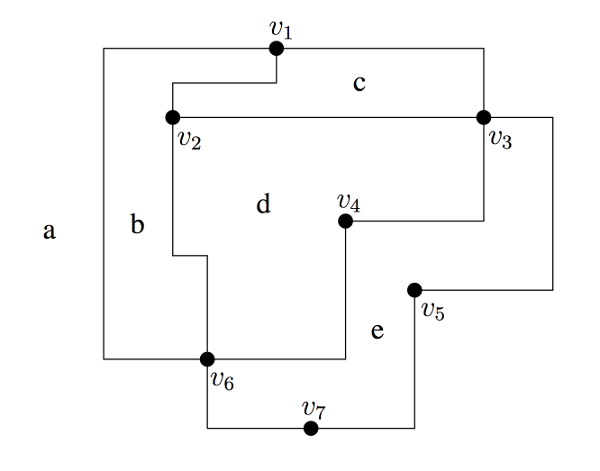
\includegraphics[scale=0.5]{img/fig3.png}
  \end{center}
  \caption{Figure 3 taken from the assignment}
\end{figure*}

In concrete terms, consider Figure 3 from the assignment text (see Figure~\ref{fig:rect-layout}).

Boundary cycle $a$ shares an edge with $b, c, e$ and has vertices $v_1, v_3, v_6, v_7$. Therefore
its polarity is
\begin{align*}
  P_a = &x_{a1} + x_{a3} + x_{a5} + x_{a6} + x_{a7} + \\
        &(z_{ab} - z_{ba}) + (z_{ac} - z_{ca}) + (z_{ae} - z_{ea}) \\
      = & 0 + 1 + 1 + 1 + 0 + \\
        & (0 - 2) + (0 - 1) + (0 - 4) \\
      = & -4
\end{align*}

Boundary cycle $e$ shares an edge with $a, d$ and has vertices $v_3, v_4, v_5, v_6, v_7$. Therefore
its polairty is
\begin{align*}
  P_e = &x_{e3} + x_{e4} + x_{e5} + x_{e6} + x_{e7} + \\
        &(z_{ea} - z_{ae}) + (z_{ed} - z_{de}) \\
      = & 1 + 1 + (-1) + 1 + 0 + \\
        & (4 - 0) + (0 - 2) \\
      = & 4
\end{align*}

Since $a$ is the outer boundary cycle and $e$ is an inner boundary cycle, the property holds as stated.

\subsection{Exercise 2.3}

The assumption that no vertex has degree greater than one is neccessary because
rectilinear layout cannot accomodate vertices of degree greater than four.

The property that no vertex has degree less than two is a logical consequence of
the requirement that there can be not cuts.

To prove that
\begin{align*}
  \sum_f x_{vf} = \begin{cases}
    0 & \text{if $v$ has degree $2$} \\
    2 & \text{if $v$ has degree $3$} \\
    4 & \text{if $v$ has degree $4$}
  \end{cases}
\end{align*}
we remember that a vertex is a member of a number of boundary cycles equal to
its degree.

We then consider the three cases:

When $v$ has degree $2$, it is
an inner turn in one boundary cycle, an an outer turn in the other, or it is
a midpoint on a straight segment. If the former, an inner turn has value $1$
and an outer turn has value $-1$, if the latter, both have value $0$, in either
case, it sums to $0$.

When $v$ has degree $3$, it is invariably an inner turn in two boundary cycles
and a midpoint on a straight segment in the third, which sums to $2$.

When $v$ has degree $4$, it is an inner turn in all four boundary cycles.

Q.E.D.

\subsection{Exercise 2.4}

\newcommand\brm[1]{\bm{\mathrm{#1}}}

Minimize $\brm c \cdot \brm z$ where
\begin{align*}
  \brm c &= [1 \quad 1 \quad 1 \quad \dots ]^\intercal \\
  \brm z &= [z_{ab} \quad z_{ac} \quad z_{ad} \quad \dots \quad z_{ba} \quad z_{bc} \quad \dots ]^\intercal,
\end{align*}
in other words $\brm z$ is the vector of all $z_{fg}$, grouped by $f$, with the outer boundary cycle
first.

Subject to $\brm A \brm z \leqslant \brm{4'} - \brm x$ and $\brm z \geqslant \brm 0$.

The structure of matrix $\brm A$ and vectors $\brm x, \brm{4'}$ requires some explanation:

Each row-vector $\brm a_f$ of $\brm A$, has the property that for the boundary cycles $f$
the scalar product $\brm a_f \cdot \brm z$ is precisely equal to $\sum_g z_{fg}$. This means that
$\brm a$ is mostly $0$'s, but with a single run of consequtive $1$'s in it, to `select' precisely
the collection (over $g$) of $z_{fg}$ to sum.

The vector $\brm{4'}$ has as its first entry $ -4$ and $4$ for all the remaining entries.

The vector $\brm x$ has as its entries $\sum_v x_{vf}$ for each boundary cycle $f$, in the same
ordering of boundary cycles as in $\brm z$

In essence, when computing $\brm A \brm z$, one computes precisely  $\sum_g z_{fg}$ for each
boundary cycle $f$.

We remember that for all boundary cycles $f$ the following holds
\begin{align*}
  \sum_g z_{fg} + \sum_v x_{vf} &= \pm 4 \\
  \sum_g z_{fg} &= \pm 4 - \sum_v x_{vf}
\end{align*}
(with $-4$ only when $f$ is the outer boundary cycle)
which is precicely equivalent to $\brm a_f \cdot \brm z = 4 - \sum_v x_{vf}$
and which can be generalized, using our above definitions, over all $f$ to precisely
$\brm A \brm z = \brm{4'} - \brm x$ which weakens to an inequality.

\subsection{Exercise 2.5}

We have one strategy that yielded no results, and one that did. We showcase
both because we wrote up the first one before discovering it wasn't usable,
and because we are proud of our work.

\subsubsection{REBM $\to$ LP $\leftrightarrow$ MCFP}

Perhaps it is possible to convert both problems to LP, use the
LP-MCPF as a template to convert LP-REBM into a similar form, LP-REMB$\prime$
and then turn that into an instance of MCPF.

MCFP is formulable as a canonical LP problem as follows:

In MCFP, we denote the demand as $d$, the cost function over edges as $a(\cdot,\cdot)$, the
capacity as $c(\cdot,\cdot)$ and the flow as $f(\cdot, \cdot)$.

Minimize
\begin{align*}
  \brm a \cdot \brm f
\end{align*}
subject to
\begin{align*}
  \brm A \brm f &\leqslant \brm b \\
  \brm f \geqslant \brm 0
\end{align*}

Choose an arbitrary ordering of edges and let
\begin{align*}
  \brm a = [a(v_1,v_2)\quad a(v_1,v_3) \quad \dots 0]^\intercal
\end{align*}
be the cost of each edge in that order; let
\begin{align*}
  \brm f = [f(v_1, v_2)\quad f(v_1,v_3) \quad \dots 1]^\intercal
\end{align*}
denote the flow over each edge in order.

The constraints $\brm A$ and $\brm b$ have the flollowing form:
\begin{align*}
  \brm b = [0\quad \brm c\quad \brm 0]
\end{align*}
where
\begin{align*}
  \brm c = [c(v_1, v_2)\quad c(v_1,v_3)\quad \dots]^\intercal
\end{align*}
is the constraints in order, and the $\brm 0$ vector has length
equal to the number of vertices in the graph.

The matrix $\brm A$ has three kinds of rows:

The first row is $1$'s for all edges that exit the source and $0$ otherwise,
except for the last entry which is $-d$. This means we sum the flows out of the source,
and require them to be exactly equal to $d$.

The next run of rows is an identity matrix, with each row picking out exactly 
one flow, which is then compared to the run of capacities, $\brm c$ inside $\brm b$.

The last run of rows is one row for each vertex, with $1$'s for exactly the flows
going into a given vertex, and $-1$'s for each outgoing vertex; which is equivalent
to stating the the difference between sums of ingoing flows and outgoing flows, is $0$.

We have not found a suitable way of converting between the two LP problems.

\subsubsection{REBM $\to$ graph}

This approach is one of constructing a graph.

The first observation is that if we establish a vertex set $V = \{s, t, v_a, v_b, v_c,
\dots\}$ corresponding to the boundary cycles, and antiparalell edges between
two vertices $E = \{ (v_a, v_b), (v_b, v_a), \dots \}$ if their corresponding
boundary cycles share an edge, then we can create a flow between vertices,
corresponding to the number of inner turns a boundary cycle 'pushes' into another cycle,
$f(v_a, v_b) = z_{ab}$.

(Note: the usual methods of eliminating antiparallel edges are applicable.)

It can then be shown that there needs to exist edges from the source $s$ to each
vertex $v_b$ that corresponds to an inner boundary cycle, and an edge to the
sink $t$ from the vertex $v_a$ corresponding to the outer boundary cycle, in
order to satisfy the requirement for flow conservation.

The capacity $c(v_b, v_c)$ for each edge $(v_b, v_c)$ is the maximum number of
inner turns that can by geometric feasibility be put on an edge. We can create
an arbitrary number of inner turns in any edge by `twisting' a given vertex
of the embedding, turning the edges into it into a right-angled spiral. Ergo
$c(v_b, v_c) = \infty$.

The demand is, for the outer boundary cycle $a$, the number of outer turns $\sum_f z_{af}$ needed to
satisfy the geometric feasibility constraint
\begin{align*}
  \sum_f z_{af} + \sum_v x_{va} = -4
\end{align*}

The cost function is trivial.
